\chapter{Tag Clouds}
\label{sec:tagclouds}

Tagging, which is one of the defining characteristics of Web 2.0 services, allows users to collectively classify and find information. Some websites include tag clouds as a way to visualize tags in a folksonomy.(4)\\

An empirical analysis of the complex dynamics of tagging systems, published in 2007,(5) has shown that consensus around stable distributions and shared vocabularies does emerge, even in the absence of a central controlled vocabulary.For content to be searchable, it should be categorised and grouped. This is possible only if the content is tagged like keywords in a journal article.\\

(4) Lamere, Paul (June 2008). "Social Tagging And Music Information Retrieval". Journal of New Music Research 37 (2): 101�114. http://www.informaworld.com/smpp/content~db=all~content=a906001732. \\
(5) Harry Halpin, Valentin Robu, Hana Shepherd The Complex Dynamics of Collaborative Tagging, Proceedings of the 16th International Conference on the World Wide Web (WWW'07), Banff, Canada, pp. 211-220, ACM Press, 2007. \\

We have found so far no other application implementing LSA in order to present an overview of the main topics found in a collection of unstructured texts, based on user queries. The TagCloud Summarizer is in this sense new.\\

There exist, however, search engines, which utilize categorizing of search results, such as Yippy(former Clusty, Vivisimo). It utilizes search, classification, and Social web (Web 2.0).
\section{existing implementations}
http://cloud.yippy.com/  - visualizes topics based on search queries. Created at Vivisimo company, also creator of one of the most successful meta search engines, offering classification of search results, Clusty (Vivisimo). \\

SenseBot Summarizer summarizes search results in the form of a tag cloud.\\

Google on the other hand offers "Wonder wheel" option, in order to display search results \\ 

TagCloud Summarizer is a tool that users can use to instantly visualize a topic using the familiar tag cloud display. Users can create a cloud based on a query.\\

TagCloud Summarizer generates a cloud using the user's search results for the topic they enter. Using the Summarizer to generate the cloud also ensures that it is always up-to-date because topics/main concepts are generated in real-time, based on the user's query.\\

\section{use}
Use the TagCloud Summarizer for online web-pages, search systems, or personal web-sites.\\

\begin{summary}
This chapter presents an overview of tagclouds used as a method for representing text content.
\end{summary}

Tag Clouds are popular applications used for vaious purposes: as a navigation mechanism, as indicators of activity within social media experiences, for visualization in texts and textual data, for annotation of documents~\ref{fig:tagcloud}. The importance or weight of words in the tag cloud are shown with size of font and/or color. The tag clouds are hyperlinks leading to a collection of items associated with the tag.\\
A version of tag cloud is called text cloud. It is used as a visual display that conveys the broad themes that emerge from textual analysis.  
There are three types of tag clouds depeding on their purpose and use. The first type contains a tag represeting the frequency of each term. The second type is a global tag cloud whose tags has frequencies aggreggated over all items and users. The third type of tag cloud contains categories, and its tags' size indicates the number of subcategories.\\
%TODO
%generate a tag cloud based on the contents in docmachine!!!!!!! replace the figure
%
% Opencloud
%
\begin{figure}[htbp]
	\centering
	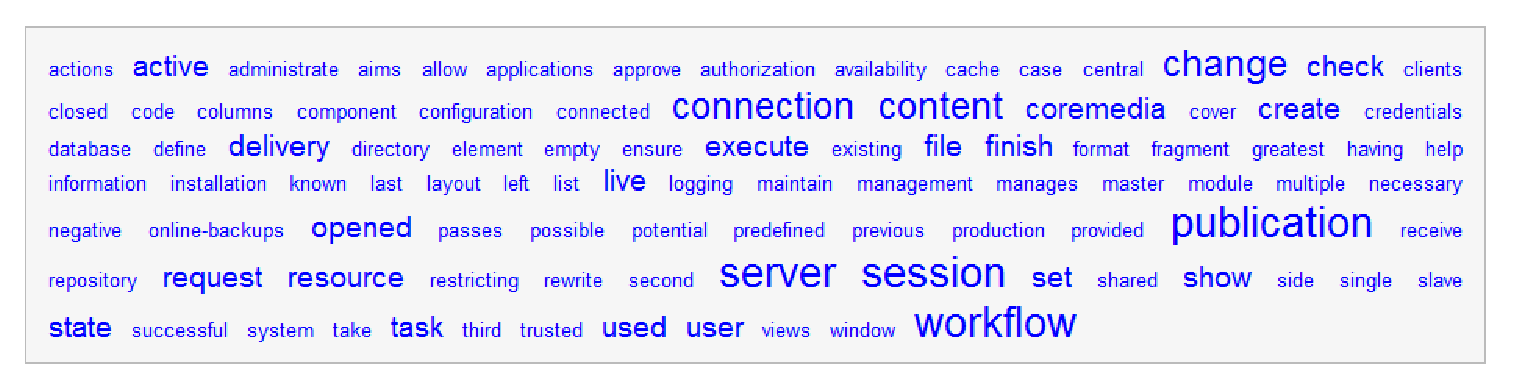
\includegraphics[width=\ScaleIfNeeded]{img/tagcloud} 
 % or [scale=0.5]
	\caption{Tag Cloud}
	\label{fig:tagcloud}
\end{figure}

\section{1}
\label{sec:semannot:1}
Related work \\
Opinion Crawl\footnote{\url{http://www.opinioncrawl.com/}} - web sentiment analysis application. It generates a concept cloud from daily scanned blogs, web site articles. \\

SenseBot Search Results Summarizer is a plugin for Mozilla Firefox browser that generates a tag cloud of the main concepts returned as search results from Google. \\

Search Cloudlet\footnote{\url{https://addons.mozilla.org/en-US/firefox/addon/9943/}} is another Firefox Addon that inserts a related tagcloud into Google interface. Working behind the scenes, Search Cloudlet injects a tag cloud of related words in to both Google and Yahoo search results pages. Then you can use the tag links to quickly and easily filter and refine your searches.



LinkSensor
SenseBotSummarizer
All three are based on SenseBot - a semantic search engine.
Made available from Semantic Firefox Extensions \footnote{\url{http://www.semanticengines.com/plugins.htm}}\\

\section{Brainstorming}
What is a tag cloud? Graphical representation of a collection of tags. Tag clouds visualize word frequency in a given text.\\

Tag clouds may be used as a topic summary.\\

There are three main types of tag cloud applications used in social software.\\
\begin{enumerate}
\item frequency of items / tags
\item number of items to which a tag has been applied
\item tags are categorization method for content items 
\end{enumerate}
The following tag clouds were evaluated in order to select the solution that is most applicable for Tag Cloud Summarizer project.\\
\begin{itemize}
\item Yippi Cloud Creator (former Clusty) \footnote{\url{http://cloud.yippy.com/}}
\item TagsTreeMaps\footnote{\url{http://tagstreemaps.sourceforge.net/TagsTreeMaps.html}}
\item OpenCloud\footnote{\url{http://opencloud.sourceforge.net/}}
\end{itemize}

\section{Tag clouds construction}
According to \cite{hoppe:2010}: \\
Erstellung von Schlagwortwolken
Tagging beschreibt die Aktivit�t, eine Ressource mit einem oder mehreren Schl�sselworten
oder Schl�sselphrasen zu assoziieren. Ein Tag ist als Etikett oder Notiz zu verstehen,
um zu einem sp�teren Zeitpunkt Dinge leichter wieder finden zu k�nnen. Tags dienen
somit der Organisation von Ressourcen.
Gro�er Beliebtheit erfreuen sich unter anderem kollaborative Tagging-Dienste wie
Flickr (Bilder), del.icio.us (Internetseiten) oder Facebook (soziales Tagging). Beim kollaborativen
Tagging annotieren Nutzer selbst die entsprechenden Ressourcen. Der auf diese
Weise implizit entstehende sogenannte tagspace soll anschlie�end effizient durchsuchbar
sein. Jedoch f�hrt das manuelle Annotieren von Ressourcen zu Problemen, wie Golder
u. Huberman (2006) aufzeigen. Synonyme und Polyseme verursachen dabei Probleme,
die bereits in Kapitel 2.1.1 angesprochen wurden. So schlie�t eine Bildersuche mittels
des Schl�sselworts Auto keine Bilder mit ein, die nur mit dem Synonym Pkw assoziiert
sind. Ein weiteres Problem ist, das dieselben Ressourcen von verschiedenen Nutzern unterschiedlich
annotiert werden. F�gt ein Nutzer als Schl�sselwort einem Bild Auto als
Schl�sselwort hinzu, so wird ein anderer durch Zuweisung von Volkswagen Golf Mk5
(A5/Typ 1K, 2003-2009) deutlich konkreter.
Um Inkonsistenzen bei der Zuweisung von Tags zu vermeiden und dadurch die Retrievalqualit�t
von Suchmaschinen zu steigern, wird automatisches Tagging eingesetzt.
Dieses dient vor allem beim Annotieren von neuen Weblog-Nachrichten dazu, Empfehlungen
f�r passende Schl�sselworte einem Nutzer vorzuschlagen.
Brooks u. Montanez (2006) annotieren automatisch neue Nachrichten in Weblogs. Sie
verwenden dazu die drei h�ufigsten Terme einer Nachricht, gewichtet nach dem tf-idf -
Schema. Nachteil ist, dass Schl�sselworte somit auf Wort-Unigrammen und dem der
Nachricht zugrundeliegenden Vokabular beschr�nkt sind.
Mishne (2006) ermitteln zu neuen Nachrichten in Weblogs zun�chst �hnliche Nachrichten,
die von anderen Nutzern zuvor verfasst wurden. Anschlie�end werden einem Nutzer
die dort verwendeten Schl�sselworte als Tags f�r eine neue Nachricht vorgeschlagen.
Lee u. Chun (2007) setzen dagegen ein �berwachtes Lernverfahren ein � ein neuronales
Netz. Dieses wird auf einer Menge von Blog-Nachrichten trainiert, denen Tags zugewiesen
sind. Anschlie�end k�nnen Empfehlungen f�r Tags f�r neue Nachrichten gegeben werden.
Grundlage zur Erfassung von Tags sind Verfahren der Schl�sselwortbestimmung. Dabei
werden h�ufige, durch tf-idf gewichteteWort-Bigramme in den Nachrichten ermittelt. Ob
die ermittelten Bigramme auch allgemein h�ufig verwendet werden, wird anschlie�end
mittels WordNet evaluiert.
Neben der automatischen Empfehlung von Schl�sselworten wird ebenso versucht, aus
dem tagspace eine Hierarchie abzuleiten (Brooks u. Montanez, 2006; Wu u. a., 2006).
Solche Hierarchien dienen der Suchoptimierung. Da im Allgemeinen bei der Erstellung
von Schlagwortwolken auf vorhandene Schl�sselworte zur�ckgegriffen wird, finden sich
bis auf die Erstellung von Taxonomien aus Schlagworten keine Gemeinsamkeiten mit
Ans�tzen des Cluster-Labelings. 
